% !TEX TS-program = pdflatex
% !TEX encoding = UTF-8 Unicode

% This is a simple template for a LaTeX document using the "article" class.
% See "book", "report", "letter" for other types of document.

\documentclass[12pt]{article} % use larger type; default would be 10pt

\usepackage[utf8]{inputenc} % set input encoding (not needed with XeLaTeX)

\usepackage{tikz}


%%% Examples of Article customizations
% These packages are optional, depending whether you want the features they provide.
% See the LaTeX Companion or other references for full information.

%%% PAGE DIMENSIONS
\usepackage{geometry} % to change the page dimensions
\geometry{a4paper} % or letterpaper (US) or a5paper or....

\usepackage{graphicx} % support the \includegraphics command and options

%%% PACKAGES
\usepackage{booktabs} % for much better looking tables
\usepackage{array} % for better arrays (eg matrices) in maths
\usepackage{paralist} % very flexible & customisable lists (eg. enumerate/itemize, etc.)
\usepackage{verbatim} % adds environment for commenting out blocks of text & for better verbatim
\usepackage{subfig} % make it possible to include more than one captioned figure/table in a single float
% These packages are all incorporated in the memoir class to one degree or another...

%%% HEADERS & FOOTERS
\usepackage{fancyhdr} % This should be set AFTER setting up the page geometry
\pagestyle{fancy} % options: empty , plain , fancy
\renewcommand{\headrulewidth}{0pt} % customise the layout...
\lhead{}\chead{}\rhead{}
\lfoot{}\cfoot{\thepage}\rfoot{}

%%% SECTION TITLE APPEARANCE
\usepackage{sectsty}
\allsectionsfont{\sffamily\mdseries\upshape} % (See the fntguide.pdf for font help)
% (This matches ConTeXt defaults)

%%% ToC (table of contents) APPEARANCE
\usepackage[nottoc,notlof,notlot]{tocbibind} % Put the bibliography in the ToC
\usepackage[titles,subfigure]{tocloft} % Alter the style of the Table of Contents
\renewcommand{\cftsecfont}{\rmfamily\mdseries\upshape}
\renewcommand{\cftsecpagefont}{\rmfamily\mdseries\upshape} % No bold!

\definecolor{aliceblue}{rgb}{0.92, 0.97, 1.0}

\pagecolor{aliceblue}

\usepackage{background}

\usepackage{nopageno}

%%% END Article customizations

%\usepackage{mathpazo}

\usepackage{quattrocento}
\usepackage[T1]{fontenc}

\renewcommand{\sfdefault}{\quattrocentofamily}
\renewcommand{\rmdefault}{ptm}
\renewcommand{\familydefault}{\quattrocentofamily}

\linespread{1.25}

\hoffset = 35pt

\marginparwidth = 125pt
\marginparsep = 15pt
\textwidth=350pt
\textheight=625pt

\setlength{\parindent}{2em}
\setlength{\parskip}{2em}


\usepackage{titlesec}
\titleformat{\section}[hang]
{\rmfamily \huge}
{}{3em}{
    \newpage
    \rule{\textwidth}{1pt}
    \vspace{1ex}
    \centering
} % before-code
[
\vspace{-5ex}%
\rule{\textwidth}{0.3pt}
] % after-code

\titleformat{\subsection}[hang]
{\rmfamily \large}
{}{3em}{}


%%% The "real" document content comes below...

\title{{\rmfamily Introduction to Highly Scalable, Fault Tollerant, Distributed System}}
\author{RedBeardLab.github.io}
\date{} % Activate to display a given date or no date (if empty),
         % otherwise the current date is printed 

\begin{document}

\backgroundsetup{
placement=bottom,
angle=0,
color=black!40,
scale=4,
vshift=10,
contents={
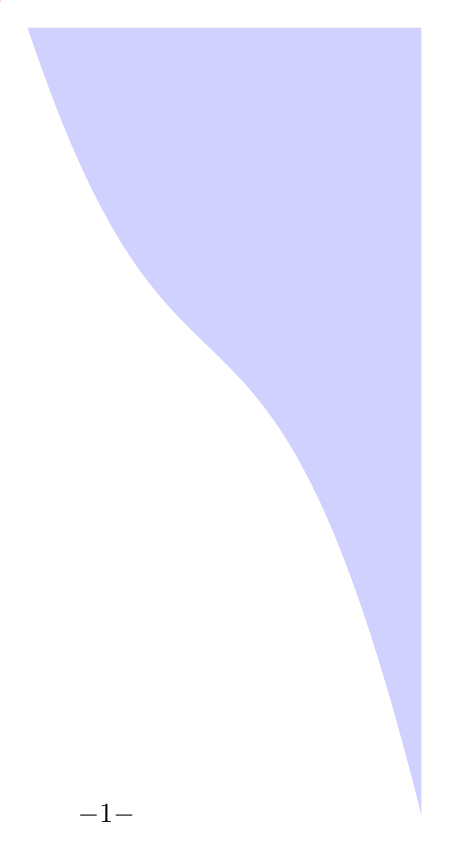
\begin{tikzpicture}
	\fill [blue!18](-5, 0) -- (0, 0) -- (0, -10) ..controls (-2, -2) and (-3, -6) ..(-5,0);
	\node at (-4, -10) {$- \thepage -$};
\end{tikzpicture}
}}

\maketitle

\newpage

{Copyright Simone Mosciatti 2016, Milano, Italy.}

This little booklet is been written hoping to serve as short, and definitely not complete nor exhaustive,  introduction to the problem and possible solution faced during the design of distributed, highly scalable, fault tolerant system.

Following the Open Source principles this work is released under the Creative Commons, contribution and suggestions are extremely welcome. 

The complete source of the project can be found at \\
{\ttfamily https://github.com/siscia/intro-to-distributed-system} \\
where contributions are encouraged.

To contact directly the author is possible to ping {\ttfamily @siscia\_} on Twitter or via email at {\ttfamily simone@mweb.biz}

\vspace{\fill}

\begin{figure}[h]
	\centering
	\includegraphics{by-sa}
\end{figure}

{\small This work is licensed under the Creative Commons Attribution-ShareAlike 4.0 International License. To view a copy of this license, visit {\ttfamily http://creativecommons.org/licenses/by-sa/4.0/} .}

\section{Introduction}

The web is exploding right now and it will keep up growing faster than ever, with it also the computing power required and the networking necessities are growing.

However our computers are not getting much faster, they have reached their physically limit regarding performance, fortunately those machines are getting cheaper and more power efficient every single day.

The next logical step is to used a lot of cheap, small and power efficient computers instead of a few, big, expensive ones.

Computation is going to be divide between a lot of machine, likely, not even in the same datacenter, this will allow to build system that have the necessary performance for the modern web but it will also bring its own set of problems and challenges.

Build and use distributed system is know to be very hard, but why ?

\section{Why it is hard ?}

Distributed system are based on completely different foundation than traditional system, there is not a physical central point of control where all the data flow and information travel between the different part of the system in a not negligible time.

Also there is expectation that our system is live 24/7/365, using a single machine there is no way do defend ourself against power loss or somebody tripping on the cables, but if we use a lot of small machines distributed in different part of the glob there is no reason that our system should be down if some problem occur in a single datacenter.

Working in a distributed system mean that you are using more than a single machine, it is good because it means that you system could be resistant to failure, however having a lot of machines around it means that some of those will break no matter what.

Suppose that a machine goes ``down'' (whatever that means) which a small probability, lets say 1\%, this mean that a machine is ``up'' which a probability of $ 100\%-1\% = 99\%$, now suppose you have 100 machines, it means that the probability that every single machine is up at the same time is roughly $ 0.99^{100} = 0.366 $, what if you have 1000 machines ? $0.99 ^ {1000} = 0,000043171 \approx 0$ percentage of chance of having all your computer ``up''.

In a big distributed system, at any given time, some machine will be ``down'' , some other machine will be having some weird problems and -- definitely worse -- some machine that was working just fine a couple of seconds ago will go down.

To manage all this complexity and uncertainty in distributed system is necessary to use a different mental framework of the one used to build traditional systems.

	\subsection{State is evil}
	
As just discussed, no matter what, some of your machines will go ``down'', they will completely lost their memory and you will have lost the state stored in such machines.

If your system relies on some state stored in a single machine you have a single point of failure, and when -- not if -- that machine goes down your system will go in some inconsistent state.

The simplest solution is to don't keep any state in your system, but this is not always a practicable solution, keep the number of state at the bare minimum is, likely, the best trade off possible.

When you lost state you need to be sure that your system can keep operating, it can either recover the state somehow (read it back from a persistent disk, ask to other part of the system or compute it back again from some know previous state) or, if the state wasn't so important, just don't care and keep going, which is arguably a wonderful solution as long as the system is operating correctly.

	\subsection{Forget about time}
	
Different machines have different clock, they can be synchronized but it won't last.

Different clock tick at different frequencies, you simply can't relies on the time you read from one machine, especially if you want to order events.

It also important to remember that if the machines are far away from each other there is a not negligible lag between the time when you send a message from San Francisco and the time when you receive the same message in London. 

	\subsection{Order of Events}
	
If is not possible to relies on time, ordering events became harder, the only reliable way to order events is to make all the event pass through the same machine (ideally the same processor), however this doesn't scale very well.

If is necessary to order a series of events a good way is to keep a monotonic counter that can only increase and ask a new value every time is needed, doing so, however, means to keep a state, and a very important one that is not possible to loose.

	\subsection{Is not that bad}

I have been very catastrophic, but it is never that bad, most system have strict requirements about something and more relax constrained about something else. 

The chat system of a video game is not such a good deal if one message get lost, it would be nice if ever single message goes through, but if we lost one message in a million nobody will complain, however such system may need to be up 24/7 and even a couple of minutes of downtime can means a lot of lost profit.

On the other side a bank cannot afford to loose any transaction, but if your payment need a second attempt to go through is annoying but still better than loose customer moneys.

It is important to understand what part of the system can be little more relaxed and where it is necessary to be extremely robust, a technological system, even if carefully design, will always be limited, it is responsibility of the designer to make the system achieve the necessary performance.

\section{Small independent processes}

One way to build highly scalable, distributed system is to use a lot of small independent units.

These units need to be stoppable and resumable at will.

Every single one of these little units will have some responsibility and will be able to keep some sort of state.

Since we are going to need a lot of those units create a new one must be a very light, quick operation and it cannot use much memory, a operating system fork is out of the plate.

Fortunately a lot of programming languages provides something similar, those units are called process in Erlang/Elixir, tasklets or greenlets in python, Fiber in Java using Quasar or Actor using Akka, goroutines in golang and more.

I am going to refer at ``process'' from now onward.

The context switch between different processes is extremely low, almost negligible and is not problematic, similarly a process without state need very few bytes of memory.

This means that a single processor can handle an awful lot of different process while it can manage -- whit reasonable performance -- only an handful of different thread.

	\subsection{Fulfill a jar with stone or sand ?}
	
Suppose that your processor is a jar of glass, you want to use as much as possible of it, would you fulfill with weird big rocks, thread, or with fine sand, processes ?

It is clear that sand won't leave much empty space, while the rocks will leave a lot of air, unused resource, in the jar.

If you have enough processes, most of them able to do meaningful work, your CPU will be totally used, yielding a lot of performance.
	
	\subsection{Performance Bounds}

There are three main factor that can limit the performance of a system: CPU, RAM \& I/O.

A system bounded only by one of those is more desiderable because easier to scale, either vertically or horizontally.

If a system is bound only by its CPU the easiest way to manage bigger load is to use a faster processor, if the system is bound only by RAM you can buy more RAM and if a system is bound only by the I/O you can use faster disk, SSD or better network.

Similarly you can scale horizontally, distribute the computation between more machine to have better use of your CPU or RAM, use a load balancer to accommodate requests if the network is saturating, etc...

But if a system at its performance peek use the 70\% of the CPU, the IO is pretty much free and the RAM is around the 65\% there is not a clear path to sustain bigger loads.

Using small process with just a little nit of attention will make bottlenecks clearer and simpler to spot.

	\subsection{Isolation and message passing}
	
All the advantages of using small process goes bust if they share memory.

If the memory is shared between processes there will be need of coordination to mutate the variables, coordination will slow down the execution and so it is preferable to let every process have it own independent memory.

Process cannot share memory, but the need to communicate somehow, usually this is implemented via message.

A message is send from a process to another and left on the receiver mail box, the receiver will take care to look at his own mail box and take action if necessary.

Keep in mind that if you need to send some data from a process to another the data will be copied, it won't be used a reference to a common shared value.

\section{Keep minimum overhead}

Now that we have understand the advantages that small isolated process let's look at some basic rules on how to use them and the most common mistake.

There is a very simple golden path to follow when building complex system.

\begin{enumerate}
	\item Make it work
	\item Make it right
	\item Make it fast
\end{enumerate}

In order to achieve the great performances required by the modern web you need to keep testing your system and your ideas, don't have any assumptions about performance and correctness.

Said so a couple of suggestions:

	\subsection{Avoid single process bottlenecks}
	
One of the simplest way to make a system speedup is to get rid of your bottlenecks, if all the process in your system need to communicate with a single process, in order to coordinate, or to look at some global value, that single process is, or is about to be, your bottleneck.

You need to design your system trying to avoid such bottlenecks as much as possible.
	
	\subsection{Keep it as simple as possible}

A lot of languages provide some sort of framework to build application, in Erlang it would be OTP, they are very helpful to build any meaningful application but they come with some overhead that not always is necessary.

You need to know very well both the framework you are using and the language primitives so that you can always choose the smallest sufficient element to get the job done.

	\subsection{Don't couple elements together}

Ideally you want your process to have a simple and pure API, it means that it should do only one thing and that its output depends only on it input, not on some state.

Not always this is achievable, but more ``pure processes'' you have the easier will be to reason about your system and the more flexible it will be.

\end{document}
